%\documentclass[a4paper]{article}
%\usepackage[letterpaper,top=2.5cm,bottom=2cm,left=3cm,right=3cm,marginparwidth=1.75cm]{geometry}

%\documentclass[a4paper,12pt]{memoir}

\documentclass[a4paper,12pt]{article}
\usepackage[letterpaper,top=2.5cm,bottom=3cm,left=3cm,right=3cm,marginparwidth=1.75cm]{geometry}
\linespread{1.5}

\usepackage{tikz}
\usetikzlibrary{calc,backgrounds}
\usepackage{amsmath}
\usepackage{amssymb}
\usepackage{float}
%\usepackage{graphicx}
\usepackage{svg}
\usepackage{pgfplots}
\usepackage{xcolor}
\usepackage{subcaption}
\usepgfplotslibrary{fillbetween}
\pgfplotsset{compat=1.12}
%\usepackage{stackengine}

\definecolor{pale_yellow}{HTML}{ffef96}

\title{Echo State Networks}
\author{Hector Morlet \\ 22247737}
\date{\today}

%\chapterstyle{ger}

%\setlrmarginsandblock{4cm}{2cm}{*}
%\setulmarginsandblock{3.5cm}{3cm}{*}
%\checkandfixthelayout

\begin{document}

%- max 10 pages including bibliography
%- latex
%    - equations
%    - tables
%    - figures
%- well-written
%    - spelling
%    - grammar
%    - proper referencing
%        - equations
%        - tables
%        - figures
%        - citations

\maketitle

\section*{Introduction}

This paper introduces Echo State Networks and broadly covers Reservoir Computing. We begin by outlining the limitations of traditional Recurrent Neural Networks (RNNs), followed by an explanation of the defining feature of Reservoir Computers: the Echo State Property. We will establish the formalisation of a reservoir computer, and explain the structure of an Echo State Network (ESN). We will discuss how we can find adequate values for the hyper-parameters of an ESN through heuristic methods and how we can `train' our ESN using an input sequence to produce a predicted sequence.

\section*{Reservoir Computers: Background and Motivation}

A recurrent neural network is designed to perform sequence-to-sequence prediction \cite{lukosevicius2009reservoir}. RNNs are often comprised of a single `hidden layer' but can have more. The `state' value of each hidden layer is updated through the equation:

\begin{equation*}
\mathbf{s}(t+1) = \sigma (\mathbf{C_{in}} \mathbf{x}(t) + \mathbf{C_{rec}} \mathbf{s}(t) + \mathbf{\mathbf{b}})
\end{equation*}

Due to its recurrence, an RNN can approximate any sequence with arbitrary accuracy, given enough hidden layers. Fitting the parameters of an RNN requires accounting for errors propagating through time, often using the Backpropagation Through Time algorithm. However, the successive multiplication of extreme numbers (large and small) causes the gradients calculated through this algorithm to either `vanish' or `explode'\cite{lukosevicius2009reservoir}. While some RNNs such as Long Short Term Memory (LSTM) networks encode a memory buffer to mitigate this problem, reservoir computers offer another alternative.

Reservoir computers are a variation of RNNs for processing temporal data which consist of feeding input signals into a non-linear dynamical system named the `reservoir'. The parameters of the reservoir are fixed, allowing us to only fit a readout vector and avoid fitting multiple layers of hidden node weights. Thus the training algorithm can simply become regularised least squares regression, and reservoir computers can take advantage of a large number and depth of parameters without suffering from the issues of vanishing gradients. While ESNs have the added benefit of requiring far less training computation than traditional RNNs, they require some care to be taken in establishing the properties of the reservoir.



\section*{The Echo State Property}

The defining characteristic of reservoir computers is the \textit{echo state property}. This property ensures that, given a sufficiently long input sequence, the current state of the reservoir is determined uniquely by the intervening input and is independent of its initial state\cite{jaeger2001echo}. In other words, the further past inputs are from the current state, the less they impact the current state. More formally, a network possesses echo states if its states are uniquely determined by the input sequence $\mathbf{x}(t)$ for some sufficiently large $t$, i.e., $\mathbf{s}(t) = \mathbf{s}'(t)$ for any initial states $\mathbf{s}(0)$ and $\mathbf{s}'(0)$, where $\mathbf{s}(t)$ represents the reservoir state at time $t$.

%TODO fix this up

For a network to exhibit the echo state property, it must satisfy three key conditions:
\begin{itemize}
    \item \textbf{Uniform State Contraction:} The network must be contractive, meaning that differences in initial states decay over time.
    \item \textbf{State Forgetting:} The network must `forget' its initial state after a finite amount of time, ensuring that only recent inputs affect the current state.
    \item \textbf{Fading Memory:} The influence of past inputs diminishes over time, making the network's state primarily a function of recent inputs. This can be seen in Figure \ref{fig:correlation}, where the accuracy of the remembered input compared to the actual input fades as the time delay grows.
\end{itemize}

Each state of the networks can be viewed as a function of a finite sequence of prior inputs:

\begin{align}
\mathbf{s}(t) &= \mathcal{F}(\mathbf{s}(t-1), \mathbf{s}(t-2), ... \mathbf{s}(0)) \\
&\approx \mathcal{F}(\mathbf{s}(t-1), \mathbf{s}(t-2), ... \mathbf{s}(t-\tau_{MC}))
\end{align}

Where the number of time steps $\tau_{MC}$ corresponds to some memory capacity of the network. The states that are beyond $\tau_{MC}$ steps in the past practically do not contribute to $\mathbf{s}(t)$. The memory capacity for a given time delay $\tau_{max}$ can be quantified by the following method :

\begin{equation*}
MC(\tau_{max}) = \sum^{\tau_{max}}_{\tau=1} correlation\bigg(\{\mathbf{x}(n-\tau), \mathbf{y}_\tau(n)\}_{n=\tau}^{n=T}\bigg)
\end{equation*}

The variable $\mathbf{y}_\tau$ refers to the output of a reservoir computer trained to reproduce the input from $\tau$ time steps in the past. We are calculating the correlation of these `remembered' values with the actual values over the whole sequence, where T is the final time step of the sequence. Figure \ref{fig:correlation} shows correlations measured for a reservoir computer over a range of $\tau$ values. To produce the memory capacity for a particular time delay $\tau_{max}$, we then sum the correlations calculated for time steps 1 to $\tau_{max}$. Figure \ref{fig:memory_capacity} shows the relevant memory capacities for the measured correlations. The reader may notice that Figure \ref{fig:memory_capacity} is a cumulative sum of Figure \ref{fig:correlation}. To measure the length of the reservoir computer's memory $\tau_{MC}$, we should find the lowest value of $\tau_{max}$ for which the memory capacity has converged. This value will represent how far back a reservoir computer can recall patternless inputs. We can see an example of this convergence in the memory capacity in Figure \ref{fig:memory_capacity}. In this example, the memory capacity converges to around 11 after approximately $\tau_{max} = 27$, so we can say that $\tau_{MC} \approx 27$.


\begin{figure}
\centering
\begin{subfigure}{.5\textwidth}
  \centering
  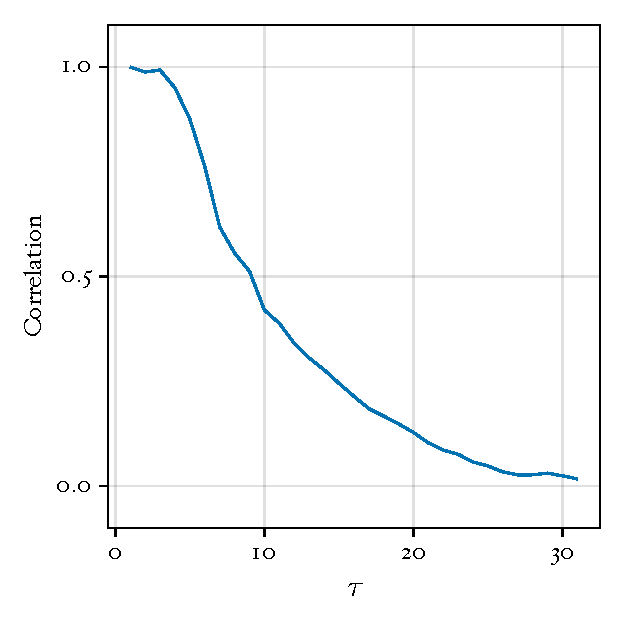
\includegraphics[width=\linewidth]{correlation}
  \caption{Correlation over $\tau$}
  \label{fig:correlation}
\end{subfigure}%
\begin{subfigure}{.507\textwidth}
  \centering
  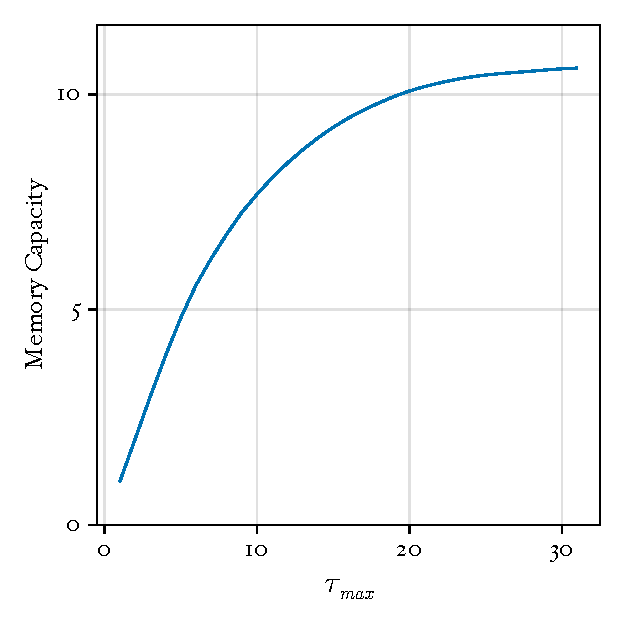
\includegraphics[width=\linewidth]{memory_capacity}
  \caption{Convergence of memory capacity $MC(\tau_{max})$}
  \label{fig:memory_capacity}
\end{subfigure}
\caption{Measures of correlation and memory capacity over time delay $\tau$ for an example reservoir computer, an Echo State Network with 100 nodes and $\rho=2$.}
\end{figure}

In most prediction tasks, the most recent inputs are more relevant than those received further back. This basic reasoning is the intuitive justification for why the echo state property is important to creating a useful model. With a large enough memory capacity, the echo state property ensures that the reservoir provides a rich, yet stable and decaying, representation of the input signal over time.

% TODO general equation description for RCs

\section*{Defining a Reservoir Computer}

Prediction using a reservoir computer can be split into two parts: firstly, the evolution of the reservoir states (also known as \emph{activation states}) and secondly, reading out the activation states to produce an output. At each time step, a reservoir computer will update its state given the input at that time step, and an output may be calculated from this state. When the time steps of the reservoir computer are discrete, we can abstractly define the state of the reservoir to be a function of the prior state and input using the evolution equation:

%TODO continuous version

\begin{equation*}
\mathbf{s}(t+1) = f_{RC}(\mathbf{s}(t), \mathbf{x}(t))
\end{equation*}

Here $\mathbf{s}(t)$ represents the state of the reservoir at time $t$, $\mathbf{x}(t)$ represents the input at time $t$ and $f_{RC}$ is the evolution operation of our reservoir.

The states $\mathbf{s}(t)$ over $t$ can then be stored as a sequence and used to fit a readout matrix $\mathbf{C}_{out}$, perhaps using a regularised least squares regression. Unseen data can then be fed into the reservoir and we can use the readout vector to glean the desired prediction from the activation states using the linear output equation:

\begin{equation*}
\mathbf{y}(t) = \mathbf{C}_{out}\mathbf{s}(t)
\end{equation*}

\section*{Echo State Networks}

Echo State Networks (ESNs) are a form of RNN introduced by Herbert Jaeger in 2001 as a part of the broader family of reservoir computing methods \cite{jaeger2001echo}. Unlike traditional RNNs, ESNs avoid the computationally expensive process of training internal weights. Instead, the internal connections of the network (which form the `reservoir') are chosen randomly and then fixed, while only the output weights are trained. This makes ESNs computationally efficient and - given the right choice of hyper-parameters - effective at processing time-dependent data.

In an ESN, the reservoir consists of a randomly generated recurrent neural network defined by the weights $\mathbf{W}_{in}$, $\mathbf{W}_{rec}$ and $\mathbf{W}_{bias}$ and activation function $f_{act}$ that together govern the evolution operation. ESNs work in discrete time, so we can define the evolution function as:

\begin{equation*}
\mathbf{s}(t + 1) = f_{act}(\mathbf{W}_{in}\mathbf{x}(t) + \mathbf{W}_{rec}\mathbf{s}(t) + \mathbf{W}_{bias})
\end{equation*}

In Figure \ref{fig:ESN}, the input weights $\mathbf{W}_{in}$ can be visualised as the connections between the input, $\mathbf{x}(t)$, and the states of the reservoir (represented as the nodes within the yellow area). The adjacency matrix $\mathbf{W}_{rec}$ is visualised in Figure \ref{fig:ESN} as the connections between states in the reservoir (the yellow area). The activation states of the reservoir $\mathbf{s}(t)$ are visualised as the nodes in the reservoir, and the readout vector, $\mathbf{C}_{out}$ is visualised as connections between the states of the reservoir and the output, $\mathbf{y}(t)$. The bias matrix $\mathbf{W}_{bias}$ also acts on the activation states, but it is not shown in Figure \ref{fig:ESN}.

\begin{figure}
\centering
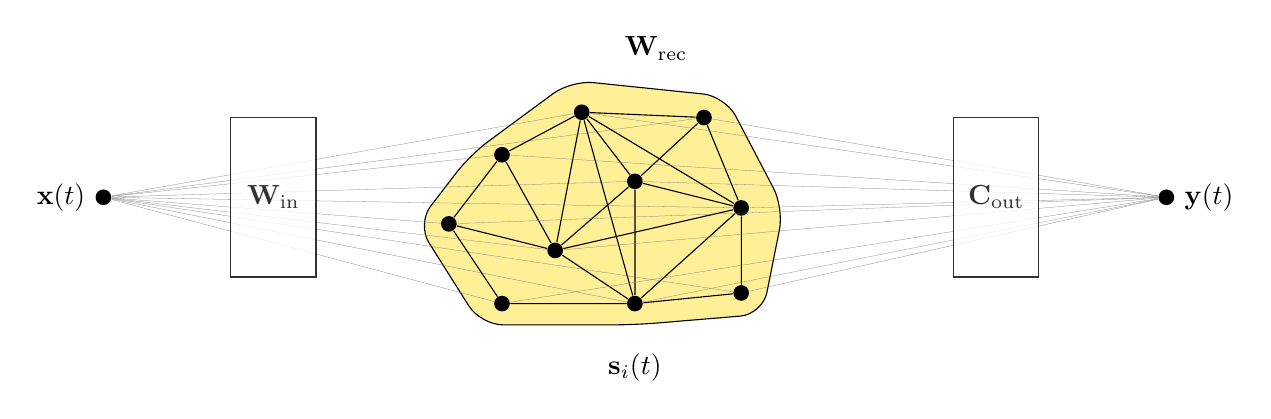
\begin{tikzpicture}[scale=1.35]
    \node[fill=black,circle,inner sep=2pt,label=left:$\mathbf{x}(t)$] (input) at (0,0) {};
    \node[fill=black,circle,inner sep=2pt,label=right:$\mathbf{y}(t)$] (output) at (10,0) {};
    
    
    \coordinate (res_anchor) at (2,3);
    \node[fill=black,circle,inner sep=2pt] (res1) at ({5-0.5},{0.8}) {};
    \node[fill=black,circle,inner sep=2pt] (res2) at ({5},{-1}) {};
    \node[fill=black,circle,inner sep=2pt] (res3) at ({5},{0.15}) {};
    \node[fill=black,circle,inner sep=2pt] (res4) at ({5+1},{-0.1}) {};
    \node[fill=black,circle,inner sep=2pt] (res5) at ({5-0.75},{-0.5}) {};
    \node[fill=black,circle,inner sep=2pt] (res6) at ({5-1.25},{0.4}) {};
    \node[fill=black,circle,inner sep=2pt] (res7) at ({5+0.65},{0.75}) {};
    \node[fill=black,circle,inner sep=2pt] (res8) at ({5+1},{-0.9}) {};
    \node[fill=black,circle,inner sep=2pt] (res9) at ({5-1.25},{-1}) {};
    \node[fill=black,circle,inner sep=2pt] (res10) at ({5-1.75},{-0.25}) {};

    \foreach \i in {1,...,10}
        \draw[gray,line width=0.1] (input) -- (res\i);
    
    \foreach \i in {1,...,5}
        \foreach \j in {1,...,5} {
            \ifnum\i<\j
                \draw (res\i) -- (res\j);
            \fi
        }
    
    \draw (res6) -- (res5);
    \draw (res6) -- (res1);
    \draw (res6) -- (res10);
    \draw (res10) -- (res5);
    \draw (res9) -- (res10);
    \draw (res9) -- (res2);
    \draw (res7) -- (res1);
    \draw (res7) -- (res3);
    \draw (res7) -- (res4);
    \draw (res8) -- (res4);
    \draw (res8) -- (res2);
    
    \foreach \i in {1,...,10}
        \draw[gray,line width=0.1] (res\i) -- (output);
    
    \begin{scope}[on background layer]
    \draw[draw=black,fill=pale_yellow,rounded corners=8pt]  ($(res1)+(-0.1,0.3)$) -- ($(res7)+(+0.2,+0.2)$) -- ($(res4)+(0.4,0)$) -- ($(res8)+(0.2,-0.2)$) -- ($(res2)+(0,-0.2)$) -- ($(res9)+(-0.2,-0.2)$) -- ($(res10)+(-0.3,0)$) -- ($(res6)+(-0.3,0)$) -- cycle;
    \end{scope}
    \node at (5.2, 1.4) {$\mathbf{W}_{\text{rec}}$};
    \node at (5, -1.6) {$\mathbf{s}_i(t)$};
    
    \draw[fill=white,opacity=0.8] (1.2,-0.75) rectangle (2.0,0.75) node[midway] {$\mathbf{W}_{\text{in}}$};
    \draw[fill=white,opacity=0.8] (8, -0.75) rectangle (8.8,0.75) node[midway] {$\mathbf{C}_{\text{out}}$};
\end{tikzpicture}
\caption{A diagram of an Echo State Network.}
\label{fig:ESN}
\end{figure}

Given a reservoir size of $k$ and an input dimension of $n$, the weights and activation function of the reservoir can be described:

\begin{itemize}
\item $\mathbf{W}_{rec}$ is a $k \times k$ adjacency matrix that defines the step-wise effect of one reservoir state on another. It is typically generated as the adjacency matrix of an Erd\H os-R\'enyi random graph with a mean degree $d$, which is then scaled to have a maximum absolute Eigenvalue of $\rho$.
\item $\mathbf{W}_{bias}$ is a bias vector of length $k$, typically generated by drawing from a uniform or normal distribution.
\item $\mathbf{W}_{in}$ is an $n \times k$ input matrix that defines the step-wise effect of the input on the reservoir state. It is also typically generated by drawing from a uniform or normal distribution.
\item $f_{act}$ is an activation function for the states; $\tanh$ is a common choice of activation function.
\end{itemize}

The performance of the ESN is determined by the dynamics of the reservoir, which is affected by our selection of `hyper-parameters' $k$, $d$ and $\rho$. These hyper-parameters are typically chosen through heuristic methods. Here we will discuss each of these hyper-parameters and common heuristic methods for choosing their values as explained by Luko{\v{s}}evi{\v{c}}ius \cite{lukosevicius2012practical}.

%TODO reference Lukoˇseviˇcius [6]


\subsection*{Reservoir Size ($k$)}

Using a large number of nodes in a traditional RNN will result in significant computational load during training, but this is less so for ESNs because the vast majority of parameters are fixed. Performance will generally improve as we increase the number of nodes, thus we can set the number of nodes in the reservoir as high as our hardware setup and inference-time requirements reasonably allow. However ESNs are not immune to the nonlinear scaling of training and inference times. As can be seen in Table \ref{tab:ks} as $k$ increases, the training and inference times increase at a nonlinear rate. To summarise, a larger number of nodes will result in better performance and ESNs with k in the hundreds to thousands are common, but not without their own computation costs.

\begin{table}[h]
\centering
 \begin{tabular}{c c c c} 
 \hline
 $k$ & Mean training time (ms) & Mean inference time (ms) & $\tau_{MC}$\\% [0.5ex] 
 \hline
 10 & 1.825 & 0.498 & 4 \\ 
 20 & 3.801 & 0.639 & 11 \\
 40 & 5.576 & 0.958 & 14 \\
 80 & 13.197 & 1.821 & 17 \\
 160 & 95.047 & 5.317 & 22 \\
 \end{tabular}
 \caption{Memory capacities for various values of $k$ and their training and inference times on a sequence of length 100,000.}
\label{tab:ks}
\end{table}

\subsection*{Average Degree ($d$)}

When the reservoir network is initiated using a method such as an Erd\H os-R\'enyi random graph, we can specify the average degree of the nodes. The average degree determines the sparsity of the connections within the reservoir. While it is important for $d$ to be sufficiently small so that the reservoir is sparsely connected, the literature suggests that the exact setting of this hyper-parameter is not as important as the other hyper-parameters. A typical value for $d$ is around 5\% of the total network size $k$, ensuring that the network is sufficiently sparse while still capable of capturing the dynamics of the input.

\subsection*{Spectral Radius ($\rho$)}
The spectral radius is the largest absolute eigenvalue of the reservoir's weight matrix $W_{rec}$. $\rho$ controls the dynamics of the reservoir and therefore the memory capacity of the reservoir.
If $\rho = 0$, the network is the zero matrix and so past states are not propagated through the network. In effect, the network forgets about past states and depends solely on the current input.
When $0 < \rho < 1$, the past states are propagated through the network but the current input is still the dominant effect on the activation states. As $\rho$ approaches 1, the reservoir begins to exhibit chaotic behavior. As we increase $\rho > 1$, the ESN approaches a tipping point (often referred to as the `edge of chaos') beyond which the ESN memory dominates the input signal. With values $\rho >> 1$, the ESN becomes unstable and uninformative as the input signal has little effect on its dynamics. A commonly used heuristic is to set $\rho \approx 1$ to balance the memory and the stability of the ESN, however research suggests that setting $\rho$ closer to the edge of chaos can improve performance of the reservoir.
Figure \ref{fig:memory_capacity_vs_rho} demonstrates the effect of $\rho$ on the memory capacity of the ESN. As $\rho$ is increased, memory capacity increases. Above $\rho = 1$, the spread of possible memory capacities increases considerably and the lower bound peaks at some value of $\rho$ just above $\rho=1$. We can consider this value to be the `edge of chaos', beyond which the reservoir becomes increasingly unstable and so the memory capacity becomes increasingly unreliable.

%TODO reference spectral radius graph

\begin{figure}[t]
\centering
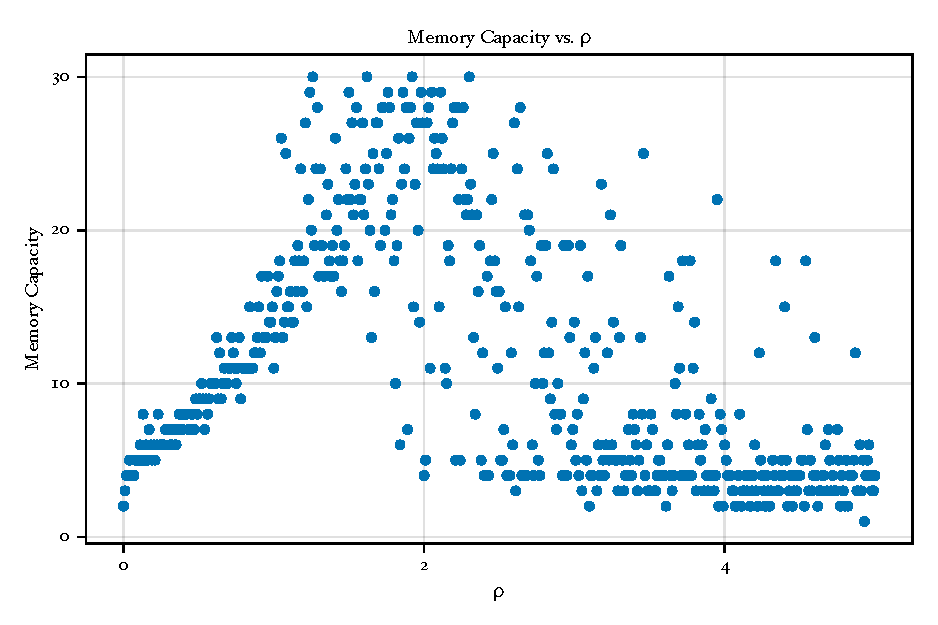
\includegraphics{memory_capacity_vs_rho}
\caption{A plot of an ESN's memory capacity for various values of $\rho$.}
\label{fig:memory_capacity_vs_rho}
\end{figure}


%TODO can include other parameters here too

\section*{Training the ESN}

Since the internal reservoir weights remain fixed, the only part of the ESN that requires training is the output weight matrix $\mathbf{C}_{out}$. This is typically done using ridge regression, also known as Tikhonov regularisation. The goal of training is to minimise the following cost function:
\begin{equation*}
\min_{\mathbf{C}_{out}} \sum_t \left\| \mathbf{y}(t) - \mathbf{C}_{out}\mathbf{s}(t) \right\|^2 + \lambda \|\mathbf{C}_{out}\|^2
\end{equation*}
where $\mathbf{s}(t)$ represents the reservoir states that were generated by feeding the training sequence into the reservoir and $\mathbf{y}(t)$ is the desired output at each time step $t$. The regularisation parameter $\lambda$ controls the degree of penalty applied to the weights.

\section*{Conclusion}

Echo State Networks have found applications in time series prediction, system modeling, and classification, but their main advantage is to handle complex, nonlinear dynamical systems with minimal computational cost. In this short paper, we have explained the background, properties and implementation of ESNs. We have discussed practical heuristics for establishing an ESN, and how hyper-parameter selection can affect the performance of the model. In my dissertation, I plan to demonstrate how novel changes to the architecture of ESNs will change their performance for tasks involving complex time series prediction.


%\cite{jaeger2001echo}
%\cite{lukosevicius2012practical}

\bibliographystyle{plain}
\bibliography{bibliography}

\end{document}
